%!TEX root = ../main.tex

%------------------------------
%  Do not add notation macros to this file
%  use notation.tex instead
%-------------------------------

%----- Theorems ----------------------------------------------------------------

%Non-LNCS theorem environments
%\newtheorem{theorem}{Theorem}
%\newtheorem{lemma}{Lemma}
%\newtheorem{corollary}{Corollary}
%\newtheorem{definition}{Definition}
%\newtheorem{example}{Example}

%This might work with amsthm
%\makeatletter
%\newtheorem{repeatthm@}{Theorem}{\bfseries}{\itshape}
%\newenvironment{repeatthm}[1]{%
%    \def\therepeatthm@{\ref{#1}}
%    \repeatthm@
%}
%{\endrepeatthm@}
%\makeatother


%LNCS related theorem environments
%\spnewtheorem*{theorem*}{Theorem}{\bfseries}{\itshape}
%\spnewtheorem*{theoremnn}{Theorem}{\bfseries}{\itshape}
%\spnewtheorem*{lemma*}{Lemma}{\bfseries}{\itshape}
%\newenvironment{claimproof}[1]{\par\noindent\underline{Proof}:\space#1}{\hfill $\blacksquare$}
\newenvironment{claimproof}[1]{%
	\def\squareforqed{$\blacksquare$}%
	\par\noindent\underline{Proof}:\space#1%
}{}
%\spnewtheorem*{definition*}{Definition}{\bfseries}{\itshape}
%\spnewtheorem{fancyclaim}{Claim}{\bfseries}{\itshape}
%\renewcommand{\qed}{\strut\hfill$\blacksquare$}

%This only works with LNCS!
% \makeatletter
% \spnewtheorem{repeatthm@}{Theorem}{\bfseries}{\itshape}
% \newenvironment{repeatthm}[1]{%
%     \def\therepeatthm@{\ref{#1}}
%     \repeatthm@
% }
% {\endrepeatthm@}
% \spnewtheorem{repeatlem@}{Lemma}{\bfseries}{\itshape}
% \newenvironment{repeatlem}[1]{%
%     \def\therepeatlem@{\ref{#1}}
%     \repeatlem@
% }
% {\endrepeatlem@}
% \spnewtheorem{repeatcor@}{Corollary}{\bfseries}{\itshape}
% \newenvironment{repeatcor}[1]{%
%     \def\therepeatcor@{\ref{#1}}
%     \repeatcor@
% }
% {\endrepeatcor@}
% \makeatother
\theoremstyle{definition}

\theoremstyle{plain}

\theoremstyle{remark}
\newtheorem{remark}{Remark}
\newtheorem{claim}{Claim}
%-------------------------------------------------------------------------------
%  Magic Stuff below
%-------------------------------------------------------------------------------

%------ Quote ------------------------------------------------------------------
\renewcommand{\quote}{\list{}{\rightmargin=\leftmargin\topsep=0pt}\item\relax}

%------ Subsection and Paragraph -----------------------------------------------
\Crefname{subsubsubappendix}{Appendix}{Appendices}%
% Saving space in case of deadlines

%\makeatletter
%\renewcommand{\section}{\abovedisplayskip 3\p@ \@plus3\p@ \@minus1\p@%
%                      \belowdisplayskip 5\p@ \@plus3\p@ \@minus1\p@%
%                      \abovedisplayshortskip 0pt \@plus2\p@%
%                      \belowdisplayshortskip 0pt \@plus2\p@ \@minus0\p@%
%                      \@startsection{section}{1}{\z@}%
%                       {-10\p@ \@plus -4\p@ \@minus -4\p@}%
%                       {6\p@ \@plus 4\p@ \@minus 4\p@}%
%                       {\normalfont\large\bfseries\boldmath
%                        \rightskip=\z@ \@plus 8em\pretolerance=10000 }}
%\renewcommand{\subsection}{\@startsection{subsection}{2}{\z@}%
%                      {-6\p@ \@plus -4\p@ \@minus -4\p@}%
%                      {2\p@ \@plus 2\p@ \@minus 2\p@}%
%                      {\normalfont\normalsize\bfseries\boldmath
%                       \rightskip=\z@ \@plus 8em\pretolerance=10000 }}
%\renewcommand{\subsubsection}{\@startsection{paragraph}{4}{\z@}%
%                      {-8\p@ \@plus -4\p@ \@minus -4\p@}%
%                      {-5\p@ \@plus -0.22em \@minus -0.1em}%
%                      {\normalfont\normalsize\bfseries\boldmath
%                      }}
\renewcommand{\paragraph}[1]{\medskip\noindent{\it #1}}
%\renewcommand{\paragraph}[1]{\heading{#1}}
%\renewcommand{\paragraph}{\@startsection{paragraph}{4}{\z@}%
%                      {-8\p@ \@plus -4\p@ \@minus -4\p@}%
%                      {-5\p@ \@plus -0.22em \@minus -0.1em}%
%                      {\normalfont\normalsize\bf
%                     }}
%\makeatother

%----- Comments ----------------------------------------------------------------
\RequirePackage{totcount}
\RequirePackage{color}
\RequirePackage[colorinlistoftodos]{todonotes}

\newtotcounter{notecount}
\newcommand{\notewarning}{%
\ifnum\totvalue{notecount}>0%
 \vspace{1ex}
\begin{center}
 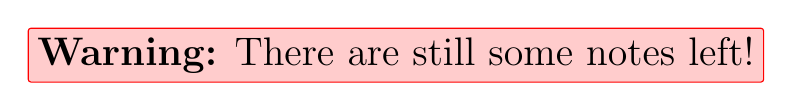
\begin{tikzpicture}[baseline=(A.south)]
    \node (A) [] at (0,0){};
    \node [rounded corners=1pt,rectangle, draw=red, fill=red!20,text=black](B) at (0.1ex,0ex){
        \Large \raggedright {\bf Warning:} There are still some notes left!
    };
 \end{tikzpicture}
\end{center}
 \vspace{1ex}
\fi
}
\makeatletter
\def\myaddcontentsline#1#2#3{%
  \addtocontents{#1}{\protect\contentsline{#2}{#3}{Section \thesubsection\ at p. \thepage}{}}}

\ifWorkInProgress
\renewcommand{\@todonotes@addElementToListOfTodos}{%
    \if@todonotes@colorinlistoftodos%
        \myaddcontentsline{tdo}{todo}{{%
            \colorbox{\@todonotes@currentbackgroundcolor}%
                {\textcolor{\@todonotes@currentbackgroundcolor}{o}}%
            \ \@todonotes@caption}}%
    \else%
        \myaddcontentsline{tdo}{todo}{{\@todonotes@caption}}%
   \fi}%
\newcommand*\mylistoftodos{%
  \begingroup
       \setbox\@tempboxa\hbox{Section 9.9 at p. 99}%
       \renewcommand*\@tocrmarg{\the\wd\@tempboxa}%
       \renewcommand*\@pnumwidth{\the\wd\@tempboxa}%
       \listoftodos%
  \endgroup
}
\fi
\makeatother
\definecolor{lightgreen}{rgb}{0.86, 0.93, 0.78}
\definecolor{bordergreen}{rgb}{0.55, 0.76, 0.74}
\definecolor{lightblue}{rgb}{0.70, 0.90, 0.99}
\definecolor{borderblue}{rgb}{0.01, 0.66, 0.96}
\definecolor{lightamber}{rgb}{1, 0.93, 0.70}
\definecolor{borderamber}{rgb}{1, 0.76, 0.03}
\definecolor{lightcolor4}{rgb}{ 0.93, 0.70, 1}
\definecolor{bordercolor4}{rgb}{0.76, 0.03, 1}
\definecolor{lightcolor5}{rgb}{0.78,0.86,0.93}
\definecolor{bordercolor5}{rgb}{0.74,0.55,0.76}
\newcommand{\dnote}[1]{\stepcounter{notecount}\todo[inline,bordercolor=bordergreen,linecolor=bordergreen,color=lightgreen]{\footnotesize{\sc \bf Dominik:} #1}{}}
\newcommand{\dsnote}[1]{\stepcounter{notecount}\todo[bordercolor=bordergreen,linecolor=bordergreen,color=lightgreen, fancyline]{\footnotesize{\sc \bf Dominik:} #1}{}}
\newcommand{\jnote}[1]{\stepcounter{notecount}\todo[inline,bordercolor=borderblue,linecolor=borderblue,color=lightblue]{\footnotesize{\sc \bf Jo\"el:} #1}{}}
\newcommand{\jsnote}[1]{\stepcounter{notecount}\todo[bordercolor=borderblue,linecolor=borderblue,color=lightblue, fancyline]{\footnotesize{\sc \bf Jo\"el:} #1}{}}
\newcommand{\mnote}[1]{\stepcounter{notecount}\todo[inline,bordercolor=borderamber,linecolor=borderamber,color=lightamber]{\footnotesize{\sc \bf Marta:} #1}{}}
\newcommand{\msnote}[1]{\stepcounter{notecount}\todo[bordercolor=borderamber,linecolor=borderamber,color=lightamber,
 fancyline]{{\scriptsize\sc \bf Marta:} #1}{}}
\newcommand{\enote}[1]{\stepcounter{notecount}\todo[inline,bordercolor=bordercolor4,linecolor=bordercolor4,color=lightcolor4]{\footnotesize{\sc \bf Eike:} #1}{}}
\newcommand{\esnote}[1]{\stepcounter{notecount}\todo[bordercolor=bordercolor4,linecolor=bordercolor4,color=lightcolor4, fancyline]{\footnotesize{\sc \bf Eike:} #1}{}}
\newcommand{\tnote}[1]{\stepcounter{notecount}\todo[caption={},inline,bordercolor=bordercolor5,linecolor=bordercolor5,color=lightcolor5]{\footnotesize{\sc \bf Tal:} #1}{}}
\newcommand{\tsnote}[1]{\stepcounter{notecount}\todo[caption={},bordercolor=bordercolor5,linecolor=bordercolor5,color=lightcolor5, fancyline]{\footnotesize{\sc \bf Tal:} #1}{}}

%----- Algorithm Environment ----------------------------------
\RequirePackage[noend]{sty/algpseudocodex}
%Header for Algorithms/Functionalities
\newcommand{\algoHead}[1]{\vspace{0.2em} \underline{\textbf{#1}} \vspace{0.3em}}
\newcommand{\algoHeadExt}[2]{\vspace{0.2em} \underline{\textbf{#1} #2} \vspace{0.3em}}
%Multiline Algo-States
\makeatletter
\algnewcommand{\ExtendedState}[1]{\State
\parbox[t]{\dimexpr\linewidth-\ALG@thistlm}{\hangindent=\algorithmicindent\strut\hangafter=3#1\strut}}
\makeatother
%Algorithms States
\algnewcommand\algorithmicinput{\textbf{Input:}}
\algnewcommand\Input{\item[\algorithmicinput]}
\renewcommand{\algorithmicensure}{\textbf{Output:}}
\algrenewcommand\algorithmicrequire{\textbf{Input:}}
\algrenewcommand\algorithmicensure{\textbf{Output:}}
%Algo Comments
\definecolor{commentcolor}{HTML}{6698FF}
\algrenewcommand{\algorithmiccomment}[1]{\vspace*{-.3em}{\color{commentcolor}\smash{//} #1}}
%Inline ifs
\algnewcommand{\IIf}[1]{\State\algorithmicif\ #1\ \algorithmicthen}
\algnewcommand{\EndIIf}{\unskip\ \algorithmicend\ \algorithmicif}


%----- Box Environment -----------------------------------------
% v 2019.1.DT small skips
%---
 \RequirePackage{varwidth}
 \RequirePackage{color}
 \RequirePackage[most]{tcolorbox}%with most option


%----- Protocol Boxes
 \newtcolorbox{titlebox}[5]{enhanced,halign=center,colframe=black,colback=white,boxrule={#3},arc={#2},auto outer arc,%
 %breakable,
 pad at break*=5pt,vfill before first,before={\par\smallskip\noindent},after={\par\smallskip},top=12pt,left=0pt,right=2pt,%
 enlarge top by=1pt,%enlarge bottom by=7pt,%
 fontupper=\small,
 title={\rule[-.3\baselineskip]{0pt}{\baselineskip}\sffamily\bfseries\scriptsize #1}, varwidth boxed
 title*=-30pt,
 attach boxed title to top left={yshift=-10pt,xshift=10pt}, coltitle=black,
 boxed title style={colback=white,boxrule={#5},arc={#4},auto outer arc},
 }

 \newtcolorbox{notitlebox}{enhanced,halign=center,colframe=black,colback=white,boxrule={0.5pt},arc={0.5pt},auto outer arc,
  pad at break*=5pt,vfill before first,after={\par\smallskip},left=4pt,
  attach boxed title to top left={yshift=-10pt,xshift=10pt}, coltitle=black
}

 \newenvironment{systembox}[1]
 {\vspace{\baselineskip}\begin{titlebox}{\normalsize Functionality #1}{2.5pt}{1pt}{3.5pt}{1pt}}
 {\end{titlebox}}

 \newenvironment{protocolbox}[1]
 {\begin{titlebox}{Protocol \normalfont #1}{0.5pt}{0.5pt}{1pt}{0.75pt}}
 {\end{titlebox}}

  \newenvironment{simulatorbox}[1]
 {\begin{titlebox}{\normalsize Simulator #1}{0.5pt}{0.5pt}{2pt}{0.75pt}}
 {\end{titlebox}}

  \newenvironment{gamebox}[1]
 {\begin{titlebox}{\normalsize Game #1}{0.5pt}{0.5pt}{2pt}{0.75pt}}
 {\end{titlebox}}

  \newenvironment{processbox}[1]
 {\begin{titlebox}{Process \normalfont #1}{0.5pt}{0.5pt}{1pt}{0.75pt}}
 {\end{titlebox}}

 \newenvironment{algobox}[1]
 {\begin{titlebox}{\normalsize Algorithm #1}{0.5pt}{0.5pt}{1pt}{0.75pt}}
 {\end{titlebox}}

 \newenvironment{funcbox}[1]
 {\begin{titlebox}{Function \normalfont #1}{0.5pt}{0.5pt}{1pt}{0.75pt}}
 {\end{titlebox}}

 \newenvironment{anybox}[1]
 {\begin{titlebox}{ \normalsize #1}{0.5pt}{0.5pt}{1pt}{0.75pt}}
 {\end{titlebox}}

%----- Reference magic ---------------------------------------------------------
%Enable reference of descriptions
\makeatletter
\let\orgdescriptionlabel\descriptionlabel
\renewcommand*{\descriptionlabel}[1]{%
  \let\orglabel\label
  \let\label\@gobble
  \phantomsection
  \edef\@currentlabel{#1}%
  %\edef\@currentlabelname{#1}%
  \let\label\orglabel
  \orgdescriptionlabel{#1}%
}
\makeatother

% Properly reference invariants
\newlist{invariants}{enumerate}{1}
\setlist[invariants,1]{label=\arabic*.,ref=\theinvariantsi}

\makeatletter
\if@cref@capitalise
	\crefname{invariantsi}{Invariant}{Invariants}
\else
	\crefname{invariantsi}{invariant}{invariants}
\fi
\makeatother




%----- Code markers ---------------------------------------------------------

\usepackage[noend]{sty/algpseudocodex}

% Markers
% Usage: turn on line-numbering (\begin{algorithmic}[1]) and then insert
%        \linemarker{foo} right before the line
% (Note this doesn't belong here, but neither does loading algpseudocodex
% which has precede it.)
\makeatletter
\global\def\@linemarker{}
\algrenewcommand{\alglinenumber}[1]{%
	\ifdefempty{\@linemarker}{
		\rule{7pt}{0pt}
	}{
		\rlap{
			\footnotesize\textcolor{red}{\@linemarker}:
			\global\def\@linemarker{}
		}{\rule{7pt}{0pt}}
	}
}
\algnewcommand{\linemarker}[1]{\global\def\@linemarker{#1}}

\newcommand{\refmarker}[1]{line~[\textcolor{red}{#1}]}
\newcommand{\refmarkers}[1]{lines~[\textcolor{red}{#1}]}

\newcounter{markercounter}
\newcommand\newmarker[1]{
	\stepcounter{markercounter}
	\csedef{#1}{\alph{markercounter}}
}
\makeatother

%%% Local Variables:
%%% mode: latex
%%% TeX-master: "../main"
%%% End:
